\newpage
\section{Advanced SQL}

\subsection{SQL Data Types and Schemas}
Some build-in data types in sql. 

\subsubsection{User-defined types}
\begin{itemize}
    \item Structured data types
    \item Distinct types
    \begin{lstlisting}[language=sql]
CREATE  TYPE person_name as varchar(20);
CREATE student(
    sno char(10) primary key,
    sname person_name
);
Drop TYPE person_name;
    \end{lstlisting}
\end{itemize}

\subsubsection{Create new domain}
\begin{lstlisting}[language=sql]
CREATE DOMAIN Dollars as numeric(12,2) not null;
CREATE DOMAIN Pounds as numeric(12,2);
\end{lstlisting}

Domain: Constraints, not strongly types. 

\subsubsection{Large-object types}

Large objects (e.g., photos, videos, CAD files, etc.) are stored as a large object: 
\begin{itemize}
    \item blob: binary large object --- object is a large collection of uninterpreted binary data (whose interpretation is left to an application outside of the database system). 
    \item clob: character large object -- object is a large collection of character data. 
\end{itemize}
When a query returns a large object, a pointer is returned rather than the large object itself.

e.g. 
\begin{lstlisting}[language={sql}]
CREATE TABLE students(
    sid char(10) primary key,
    photo blob(20MB),
    cv clob(10KB)
);
\end{lstlisting}


\subsubsection{Catalogs, schemas and environments}

\begin{figure}[H]
    \centering
    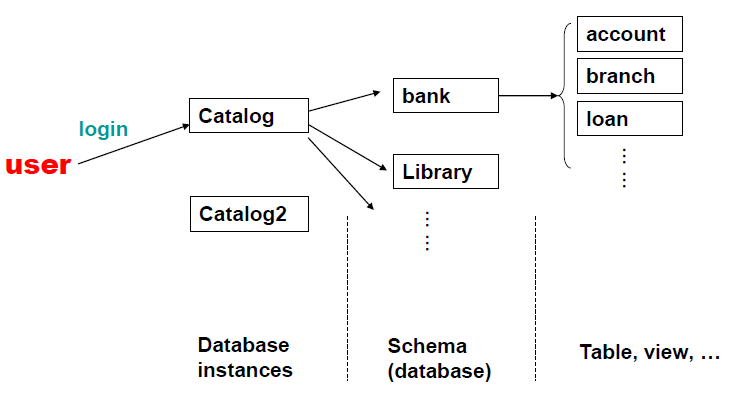
\includegraphics[width=0.479\textwidth]{DB4/Catalogs, schemas and environments}
    \caption{Catalogs, schemas and environments}
\end{figure}

\subsection{Integrity Constraints (完整性约束)}
Integrity constraints guard against accidental damage to the database, by ensuring that authorized changes to the database do not result in a loss of data consistency. 
\begin{itemize}
    \item 实体完整性、参照完整性和用户定义的完整性约束
    \item 完整性约束是数据库实例(Instance)必须遵循的
    \item 完整性约束由DBMS维护    
\end{itemize}

\textbf{Constraints on a \hl{single relation}}
\begin{itemize}
    \item Not null
    \item Primary key
    \item Unique
    \item Check($P$), where $P$ is a predicate
\end{itemize}

\subsubsection{Domain Constraints}
The \hl{check} clause in SQL-92 permits \hl{domains to be restricted}. The clause \hl{constraint value-test} is optional; useful to indicate which constraint an update violated.


\subsubsection{Referential Integrity}
\begin{definition}
    Let $r_1(R_1)$ and $r_2(R_2)$ be the relations with primary keys $K_1$ and $K_2$, respectively. The subset $\alpha$ of $R_2$ is a \hl{foreign key} referential $K_1$ in relation $r_1$, if for every $t_2$ in $r_2$ there must be a tuple $t_1$ in $r_1$ such that $t_1[K_1]=t_2[\alpha]$. Referential integrity constraints also called \hl{subset dependency}, since its can be written as 
    \[ \prod_{\alpha}(r_2) \subseteq \prod_{K_1}(r_1) \]
\end{definition}

Assume there exists relations r and s: $r$(\underline{A}, \hl{B}, C), s(\hl{\underline{B}}, D), we say attribute \hl{B} in $r$ is a \hl{foreign key} from relation $r$, and $r$ is called $referencing relation$ (参照关系), and s is called $referenced relation$ (被参照关系).

参照关系中外码的值必须在被参照关系中实际存在, 或为null.

\subsubsection{Checking Referential Integrity}
The following tests must be made in order to preserve the following referential integrity constraint: 
\begin{align*}
    \prod_{\alpha}(r_2) \subseteq \prod_K (r_1)
\end{align*}
$\alpha$ in $r_2$ is a Foreign Key. 

\textbf{Insert}: If a tuple $t_2$ is inserted into $r_2$, the system must ensure that there is a tuple $t_1$ in $r_1$ such that $t_1[K]=t_2[\alpha]$, i.e.
\begin{align*}
    t_2[\alpha]\in \prod_K (r_1)
\end{align*}

\textbf{Delete}: If a tuple $t_1$ is deleted from $r_1$, the system must compute the set of tuples in $r_2$ that reference $t_1$:
\begin{align*}
    \sigma_{\alpha=t_1[K]}(r_2)
\end{align*}
If this set is not empty, then either the delete command is rejected or the tuple in $t_2$ that references $t_1$ must themseleves be deleted (cascading deletions are possible).  

\textbf{Update}: If a tuple $t_2$ is updated in relation $r_2$ and the update modifies values for foreign key $\alpha$, then a test similar to the insert case is made. Let $t_2'$ denote the new value of tuple $t_2$, the system must ensure that 
\begin{align*}
    t_2'[\alpha]\in \prod_K(r_1)
\end{align*}

\subsubsection{Referential Integrity in SQL}
Primary, candidate keys, and foreign keys can be specified as part of the SQL create table statement:
\begin{itemize}
    \item The primary key clause lists attributes that comprise the primary key.
    \item The unique key clause lists attributes that comprise a candidate key.
    \item The foreign key clause lists the attributes that comprise the foreign key, and the name of the relation referenced by the foreign key.
\end{itemize}
\begin{lstlisting}[language={sql}]
Create table depositor(
    customer_name char(20),
    account_number char(10),
    primary key (customer_name, account_number),
    foreign key (account_number) references account,
    foreign key (customer_name) references customer
);
\end{lstlisting}


\subsubsection{Cascading Actions in SQL}
\begin{lstlisting}[language={sql}]
Create table account (
    . . .
    foreign key (branch-name) references branch
    [ on delete cascade]
    [ on update cascade ]
    . . . 
);
\end{lstlisting}



\subsubsection{Assertions}
An assertion is a predicate expressing a condition that we wish the database always to satisfy. --- for complex check condition on several relations. An assertion in SQL takes the form
\begin{lstlisting}[language={sql}]
    CREATE ASSERTION <assertion_name> CHECK <predicate>;
\end{lstlisting}
When an assertion is made, the system tests it for validity on every update that may violate the assertion.

But SQL does not provide a construct for asserting: 
\begin{align*}
    \text{for all }X, P(X)
\end{align*}
So it is achieved in a round-about fashion, using: 
\begin{align*}
    \text{not exists }X,\text{ such that not }P(X). 
\end{align*}
\begin{align*}
    \forall x P(x)=\neg \exists x \neg P(x) 
\end{align*}

e.g. 对每一笔借款, 至少有一个借款人有存款 \$ 1000以上. 

\begin{lstlisting}[language=sql, morekeywords={REFERENCES, WITH}]
CREATE ASSERTION balance_constraint CHECK(
    not exists (
        select * from loan L
        where not exists (
            select *
            from borrower B, depositor D, account A
            where L.loan_number = B.loan_number
            and B.customer_name = D.customer_name
            and D.account_number = A.account_number
            and A.balance >= 1000
        )
    )
);
\end{lstlisting}


\subsubsection{Triggers}
A trigger is a statement that is executed automatically by the system as a side-effect of a modification to the database. 

Triggering event can be insert, delete or update. Triggers on update can be restricted to specific attributes.  Values of attributes before and after an update can be referenced:
\begin{itemize}
    \item Referencing old row as: for deletes and updates
    \item Referencing new row as: for inserts and updates
\end{itemize}

\textbf{Statement Level Triggers}: Instead of executing a separate action for each affected row, a single action can be executed for all rows affected by a transaction. 
\begin{enumerate}
    \item Use for each statement instead of for each row
    \item Use referencing old table or referencing new table to refer to temporary tables (called transition tables) containing the affected rows
    \item Can be more efficient when dealing with SQL statements that update a large number of rows    
\end{enumerate}

Triggers were used for tasks: 
\begin{enumerate}
    \item Maintaining summary data
    \item Replicating databases by recording changes to special relations (called change or delta relations) and having a separate process that applies the changes over to a replica.
\end{enumerate}

\subsection{Authorization}
Security

Forms of authorization on parts of the database:
\begin{enumerate}
    \item Read authorization - allows reading, but not modification of data.
    \item Insert authorization - allows insertion of new data, but not modification of existing data.
    \item Update authorization - allows modification, but not deletion of data.
    \item Delete authorization - allows deletion of data.
\end{enumerate}


Forms of authorization to modify the database\\ schema:
\begin{enumerate}
    \item Index authorization - allows creation and deletion of indices.
    \item Resources authorization - allows creation of new relations.
    \item Alteration authorization - allows addition or\\ modifying of attributes in a relation.
    \item Drop authorization - allows deletion of relations.
\end{enumerate}

\subsubsection{Authorization and Views}
A combination of relational-level security and view-level security can be used to limit a user’s access to precisely the data that user needs.

Creation of view does not require resources authorization since no real relation is being created.

\subsubsection{Granting of Privileges}
P46

\subsubsection{Security Specification in SQL}
\begin{lstlisting}[language=sql,morekeywords={REFERENCES, WITH}]
GRANT <privilege list> ON <_table | _view>
TO <user list>
\end{lstlisting}
<user list> is:
\begin{itemize}
    \item user-ids
    \item public, which allows all valid users the privilege granted
    \item A role (more details about this later)
\end{itemize}

\subsubsection{Privileges in SQL}
\begin{enumerate}
    \item Select: allows read access to relation, or the ability to query using the view. 
    \item Insert: the ability to insert tuples.
    \item Update: the ability to update using the SQL update statement.
    \item Delete: the ability to delete tuples.
    \item References: ability to declare foreign keys when creating relations.
    \item All privileges: used as a short form for all the allowable privileges.
    \item All
    \item With grant option: Allows a user who is granted a privilege to pass the privilege on to other users.
\end{enumerate}

\subsubsection{Roles}
Roles permiting common privileges for a class of users can be specified just once, by creating a corresponding ``role''.

\subsubsection{Revoking Authorization in SQL}
The revoke statement is used to revoke authorization. 
\begin{lstlisting}[language=sql,morekeywords={REFERENCES, WITH}]
REVOKE <privilege list> ON <_table | -view>
FROM <user list> [_restrict | _cascade]
\end{lstlisting}

\subsubsection{Limitations of SQL Authorization}
\begin{enumerate}
    \item SQL does not support authorization at a tuple level.
    \item All end-users of an application (such as a web application) may be mapped to a single database user.
    \item The task of authorization in above cases falls on the application program, with no support from SQL.
\end{enumerate}

\subsubsection{Audit Trails (审计)}
An audit trail is a log of all changes (inserts/deletes /updates) to the database along with information such as which user performed the change, and when the change was performed.

\textbf{语句审计}:
\begin{lstlisting}[language=sql,morekeywords={REFERENCES, WITH}]
AUDIT <st-opt> [BY <users>] [BY SESSION | ACCESS] [WHENEVER_SUCCESSFUL | WHENEVER_NOT_SUCCESSFUL]
\end{lstlisting}
\begin{itemize}
    \item 当 BY <users> 缺省, 对所有用户审计. 
    \item BY SESSION每次会话期间, 相同类型的需审计的SQL语句仅记录一次. 
    \item 常用的<St-opt>: table, view, role, index, ...
    \item 取消审计: NOAUDIT ...(其余同audit语句)
\end{itemize}

\textbf{对象(实体)审计}:
\begin{lstlisting}[language=sql,morekeywords={REFERENCES, WITH}]
AUDIT <obj-opt> ON <obj> | DEFAULT [BY SESSION | BY ACCESS] [WHENEVER_SUCCESSFUL | WHENEVER_NOT_SUCCESSFUL]
\end{lstlisting}
\begin{itemize}
    \item obj-opt: insert, delete, update, select, grant, ...
    \item 实体审计对所有的用户起作用. 
    \item ON <obj> 指出审计对象表、视图名. 
    \item ON DEFAULT 对其后创建的所有对象起作用. 
    \item 取消审计: NOAUDIT ...
\end{itemize}

\subsection{Embedded SQL}
SQL的功能不完备性. 

A language in which SQL queries are embedded is referred to as a Host language (宿主语言), and the SQL structures permitted in the host language comprise embedded SQL.

\subsection{Dynamic SQL}
Allows programs to construct and submit SQL queries at run time.

\subsection{ODBC}

Open DataBase Connectivity (ODBC, 开放数据库互连). ODBC提供了一个公共的、与具体数据库无关的应用程序设计接口API. 它为开发者提供单一的编程接口, 这样同一个应用程序就可以访问不同的数据库服务器. 

\subsubsection{Prepared Statement}
解决sql注入